\documentclass[12pt]{article}
\usepackage{amssymb}
\usepackage{amsmath}
\usepackage{bm}
\usepackage{graphicx}
\usepackage{color, colortbl}
\usepackage{latexsym}
\usepackage{epsfig}
\usepackage{verbatim}
\usepackage{float}
\usepackage[normalem]{ulem}
\usepackage{setspace}
\usepackage{pbox}
\usepackage{color, colortbl}
\definecolor{LightCyan}{rgb}{0.88,1,1}
\usepackage[utf8]{inputenc}
\usepackage[english]{babel}
\setlength{\parskip}{2em}
\renewcommand{\baselinestretch}{1}
\usepackage{geometry}
\usepackage{newtxtext,newtxmath}
\usepackage{booktabs}
\geometry{legalpaper, margin=1in}
\usepackage{hyperref}
\usepackage{makecell}
\usepackage{caption}
\captionsetup[table]{skip=10pt}
\hypersetup{
    colorlinks=true,
    linkcolor=blue,
    filecolor=magenta,
    urlcolor=cyan,
}
\usepackage[dvipsnames]{xcolor}

\newcommand{\gc}{\cellcolor{green}}
\newcommand{\rc}{\cellcolor{Red}}
\newcommand{\yoc}{\cellcolor{YellowOrange}}
\newcommand{\oc}{\cellcolor{Orange}}
\newcommand{\sgc}{\cellcolor{SpringGreen}}
\newcommand{\yc}{\cellcolor{yellow}}
\newcommand{\tc}{\cellcolor{teal}}
\urlstyle{same}
%%%%%%%%%%%%%%%%%%%%%%%%%
\pagenumbering{roman}
\author{Osman Mamun}
\title{Development of Deep Learning Image Caption Generator}

\begin{document}
\setcounter{page}{-2}
\maketitle
\thispagestyle{empty}
\thispagestyle{empty}
\newpage
\begingroup
\def\addvspace#1{}
\tableofcontents
\endgroup
\thispagestyle{empty}
\newpage
\large
\pagenumbering{arabic}
%%%%%%%%%%%%%%%%%%%%%%%%%
\section{Introduction}
\label{Sec:intro}
%%%%%%%%%%%%%%%%%%%%%%%%%
It is relatively easy for human to be able to describe any environments they are in, e.g., when shown a photo, any human can describe very easily what's going on in the picture. This unique ability is fundamental to our existence which we use everyday, both knowingly and unknowingly, to almost every situation we encounter. Making machine enable to such ability has been an overarching goal for artificial intelligence community for a long time.

Even though there is a great progress that has been made in various computer vision tasks, such as object recognition, image classification etc., it is still a challenging task to train a computer understand an image and form a coherent sequence of word to describe the image. It is an unique challenge to solve as it unifies two different fields of machine learning, i.e., computer vision & natural language processing. Image caption generator will facilitate a lot of tasks, such as automatic captioning of items on an ecommerce website, helping blind people safely navigate the world, enabling self driving car to communicate with the passengers about an oncoming complicated situation to signal manual intervention etc.


%%%%%%%%%%%%%%%%%%%%%%%%%
\section{Data Acquisition and Cleaning}
\label{sec:dataclean}
%%%%%%%%%%%%%%%%%%%%%%%%%

For this work, we acquire two publicly available dataset, namely MS-COCO (45K images) and Flicker30K (30K images) dataset. They were downloaded using the tensorflow data download API. In the Figure \ref{fig:data_collection}, a code snippet is shown to collect data with the tensorflow API. More details about
acquiring and concatenating the data can be found in \href{https://github.com/mamunm/iamge_caption_generator/blob/main/notebooks/data_download.ipynb}{this IPython notebook}.

\begin{figure}[h!]
\begin{center}
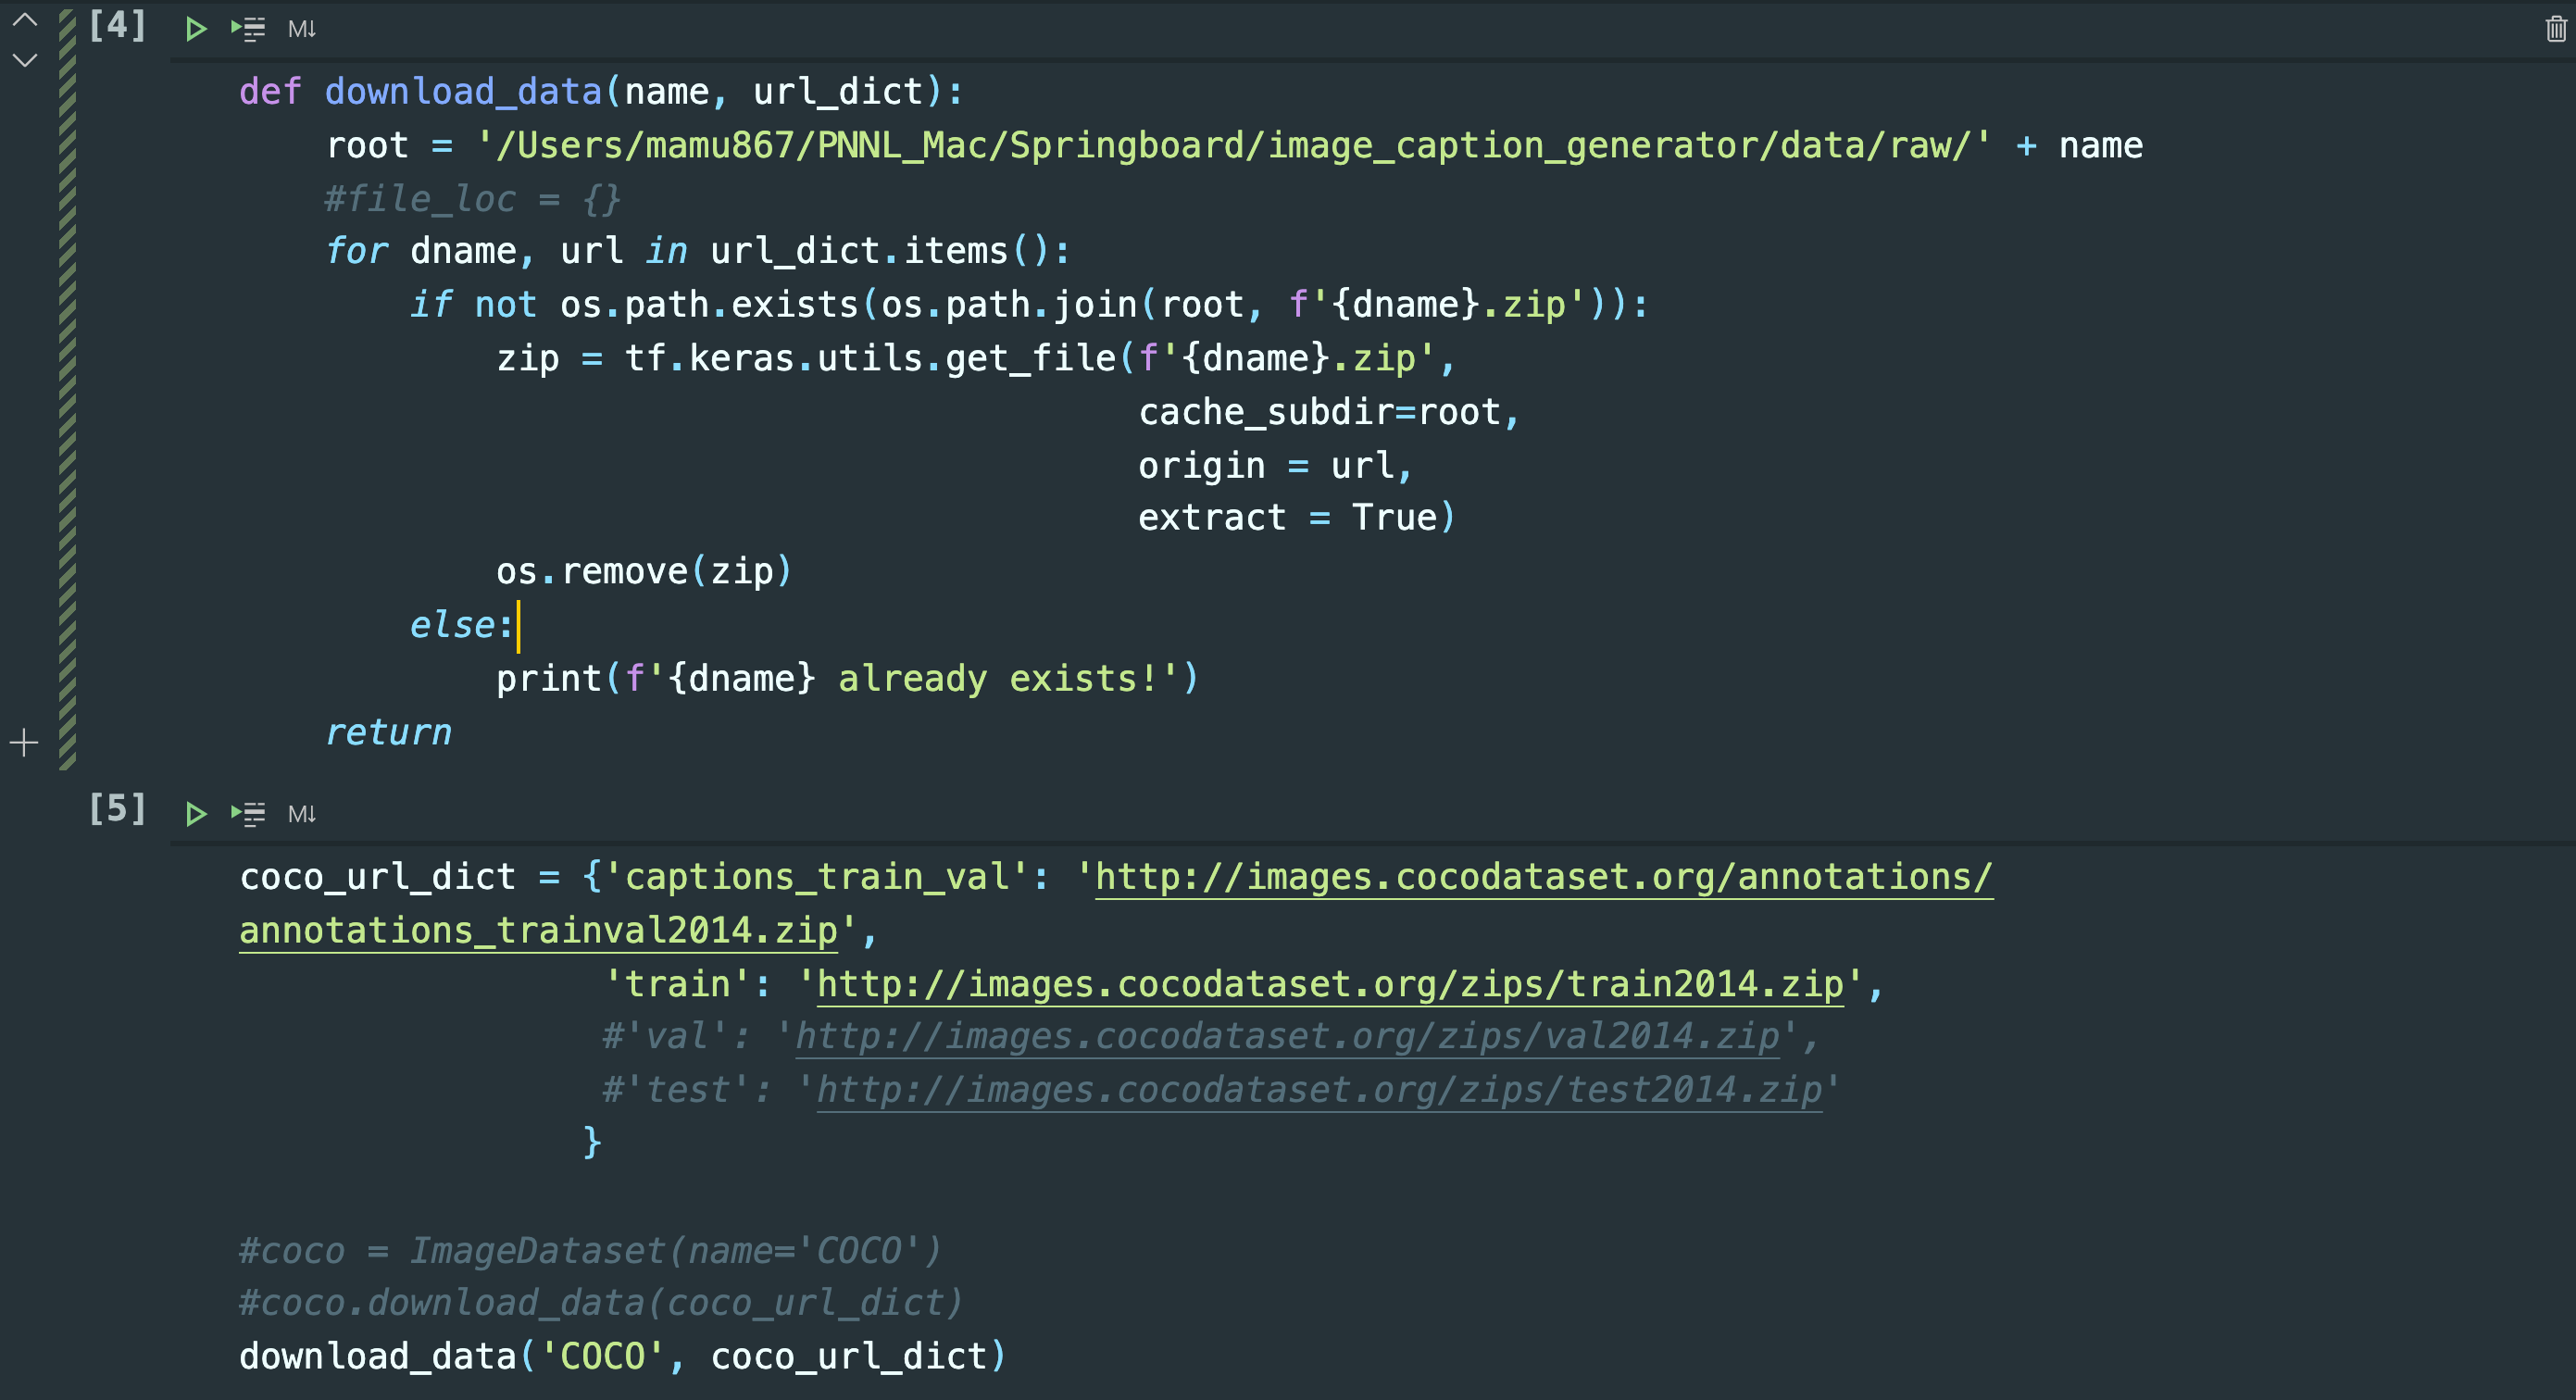
\includegraphics[width=7in]{data_collection.png}
\end{center}
\caption{\label{fig:data_collection}
Data collection for MS-COCO and Flicker30K dataset.}
\end{figure}

%%%%%%%%%%%%%%%%%%%%%%%%%
\section{Image Feature Extraction}
\label{sec:imfeat}
%%%%%%%%%%%%%%%%%%%%%%%%%

Instead of training a CNN from the scratch, pretrained image model is used to train the model. In this work, VGG16 and InceptionV3 pretrained model are used to extract the image features. The last layer of both the pretrained layer is discarded and two fully connected layers are trained on the dataset to fine-tune the model for this particular task. In Figure \ref{fig:vgg16} and \ref{fig:inceptionv3}, we show the architecture of the both model.

\begin{figure}[h!]
\begin{center}
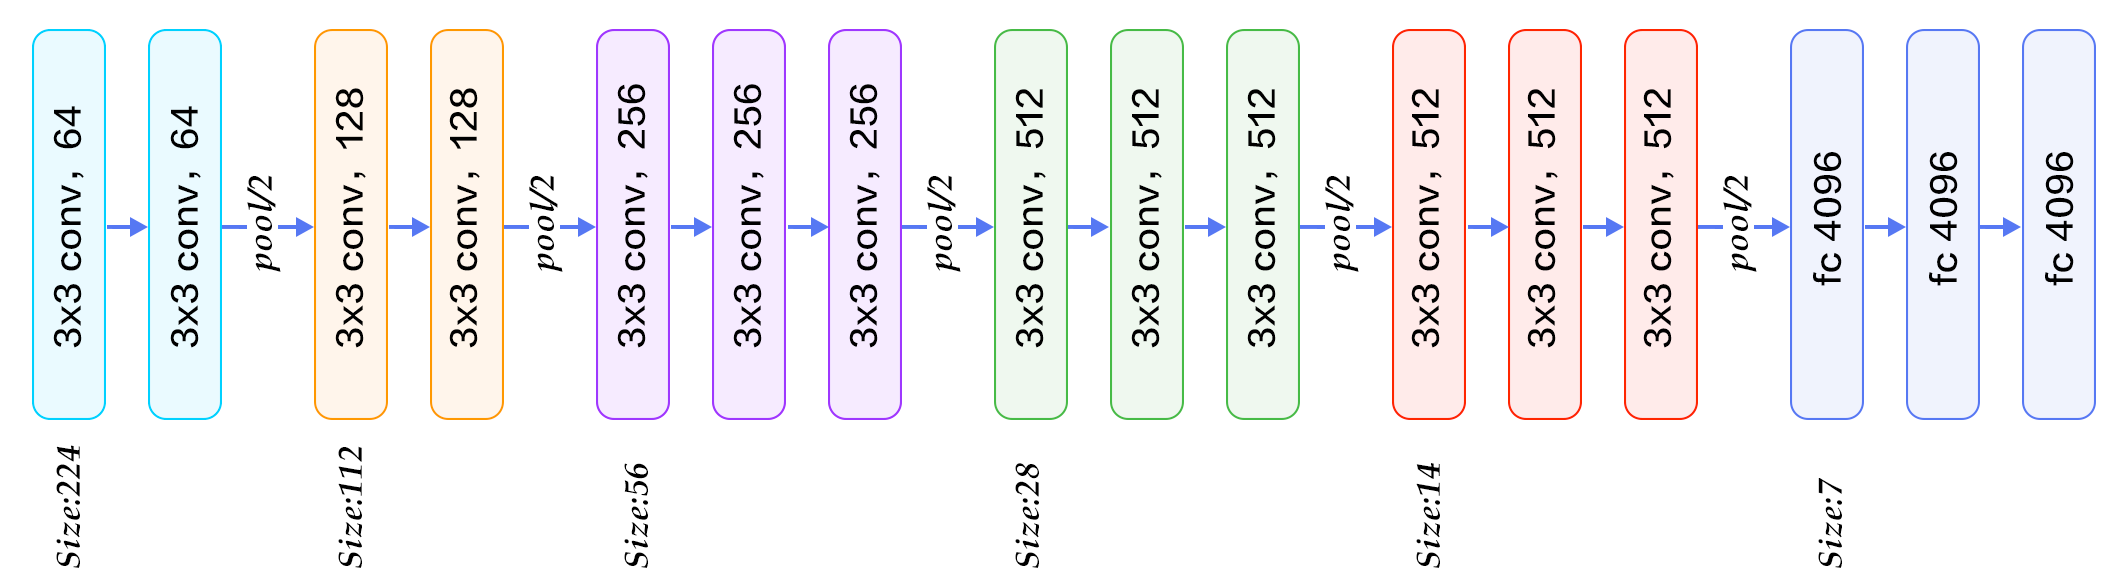
\includegraphics[width=7in]{vgg16.png}
\end{center}
\caption{\label{fig:vgg16}
Architecture of the VGG16 model.}
\end{figure}

\begin{figure}[h!]
\begin{center}
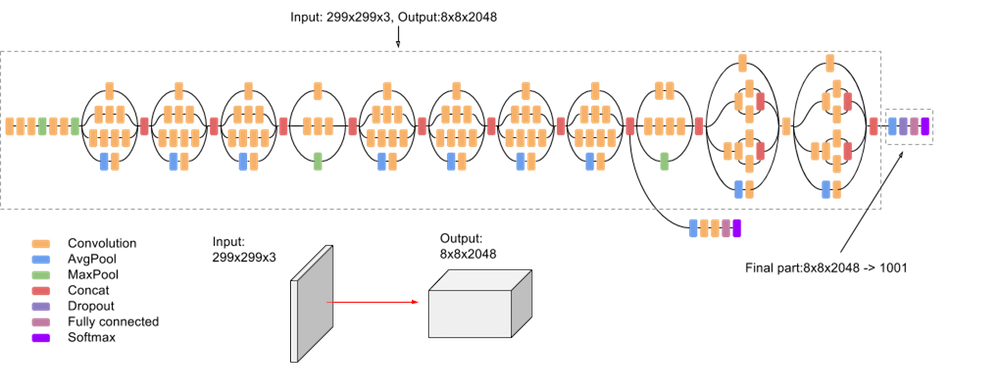
\includegraphics[width=7in]{inceptionv3.png}
\end{center}
\caption{\label{fig:inceptionv3}
Architecture of the Inception V3 model.}
\end{figure}

%%%%%%%%%%%%%%%%%%%%%%%%%
\section{Word Tokenizer}
\label{sec:imfeat}
%%%%%%%%%%%%%%%%%%%%%%%%%

Next, we used keras word tokenizer to tokenize the words in a sentence and to pad it to the maximum length of the tokenizer for this corpus. Also, <start> and <end> token is added in the beginning and end of the sentence for sequence generation process. In Figure \ref{fig:word_vec}, we show a code snippet that was used to tokenize a particular corpus. For detail description of the image feature extraction and word tokenization, we refer interested reader to \href{https://github.com/mamunm/iamge_caption_generator/blob/main/notebooks/data_processing.ipynb}{this IPython notebook}.

\begin{figure}[h!]
\begin{center}
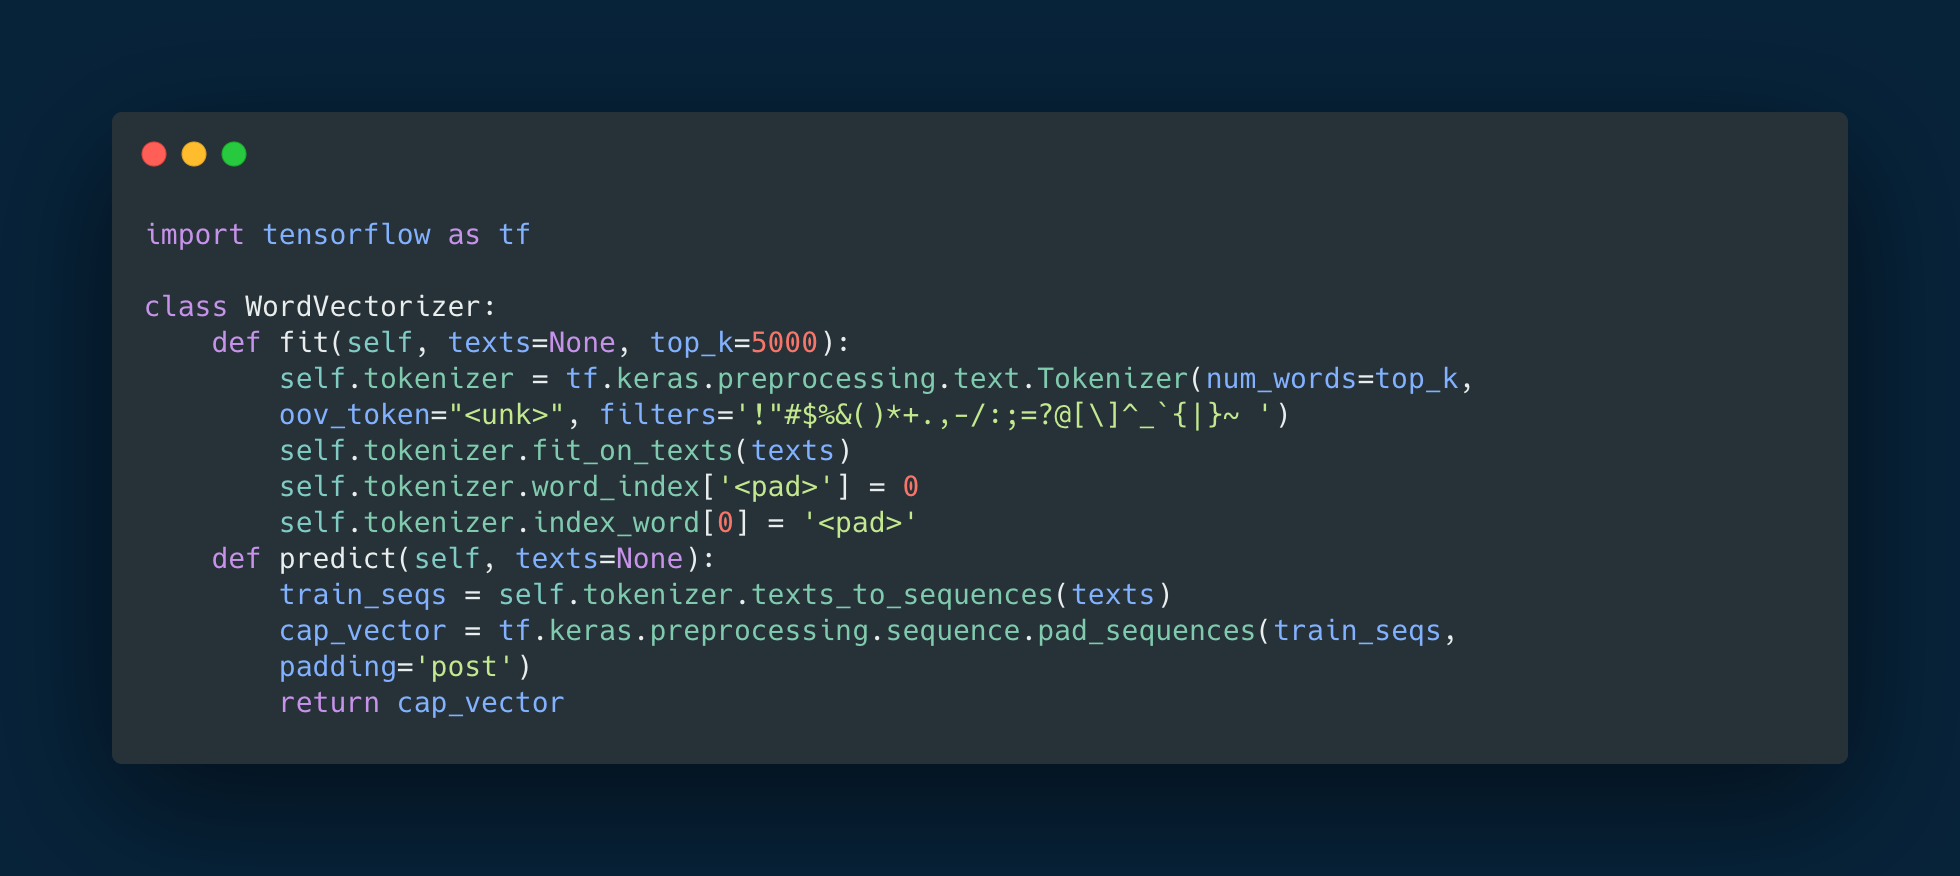
\includegraphics[width=7in]{word_vec.png}
\end{center}
\caption{\label{fig:word_vec}
Tokenization of the caption text.}
\end{figure}

%%%%%%%%%%%%%%%%%%%%%%%%%
\section{RNN Decoder}
\label{sec:imfeat}
%%%%%%%%%%%%%%%%%%%%%%%%%

For RNN decoder with attention mechanism, we used Bahdanau attention mechanism as described in the original paper by \href{https://arxiv.org/abs/1409.0473}{Bahdanau et al}. In Figure \ref{fig:BA}, an illustration of the Bahdanau attention mechanism is shown. Also, in Figure \ref{fig:decoder}, the decoder architecture used in this study is shown. We used a word embedding layer, a gated recurrent unit (GRU), and two fully conneted layer to predict the caption sequence. In the begining of the training, the decoder is fed with the image features along with the <start> token, and the model is sequentially trained to predict the next word until the <end> token is reached. In the attention, the alignment score of the previous hidden states with the new hidden states are computed and then softmaxed to identify which part of the sequence is important to find the next word in the sequence.


\begin{figure}[h!]
\begin{center}
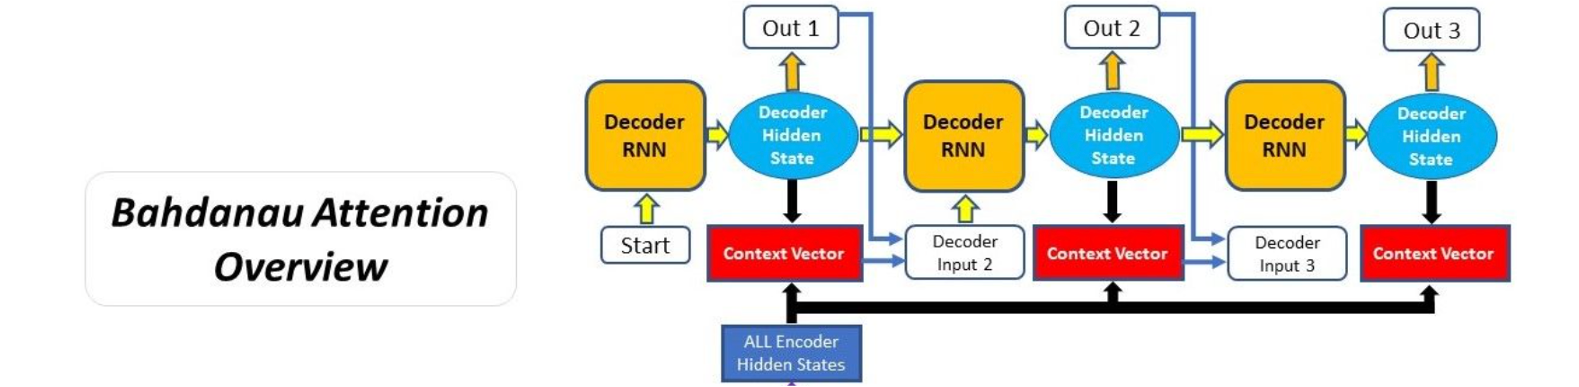
\includegraphics[width=7in]{BA.png}
\end{center}
\caption{\label{fig:BA}
Bahdanau attention mechanism.}
\end{figure}

\begin{figure}[h!]
\begin{center}
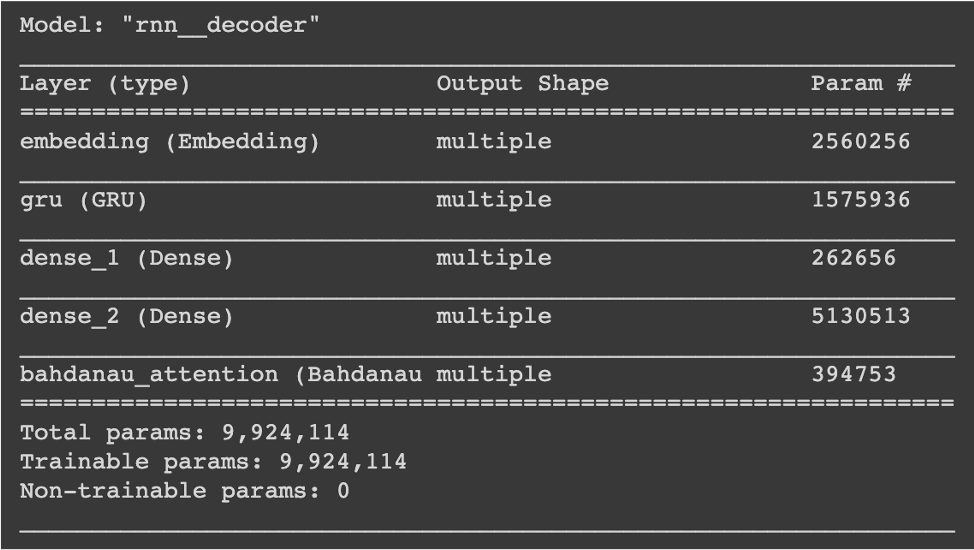
\includegraphics[width=7in]{decoder.png}
\end{center}
\caption{\label{fig:decoder}
RNN decoder to generate caption sequence from image features.}
\end{figure}


%%%%%%%%%%%%%%%%%%%%%%%%%
\section{Results & Discussion}
\label{sec:imfeat}
%%%%%%%%%%%%%%%%%%%%%%%%%

%%%%%%%%%%%%%%%%%%%%%%%%%
\subsection{Flicker30K dataset with VGG16 pretrained model}
\label{sec:imfeat}
%%%%%%%%%%%%%%%%%%%%%%%%%

We trained the Flicker30K dataset with image features derived with the VGG16 pretrained model for 20 epochs. In Figure \ref{fig:FVLR}, we can see that the loss is still going down and additional training can be done to improve the model performance. In terms of time requirements for training, the 1st epoch took about 10 minutes and the subsequent epochs took about 80 seconds on average with a GPU processor available in Google colab. In terms of training time, it's fairly reasonable time, and can be easily trained for additional $20$ epochs. It is also worth noting here that the model is trained with $12,000$ images.
In Figure \ref{fig:FV_1}, an image with the real caption "<start> a man in a white boat is rowing through fog <end>" is shown where the model predicted caption is "<start> a man in dark boat <end>". It seems like our model is pretty good at understanding the major components of an image; however, it was not particularly good at describing the fine detail in the image, e.g., fog in this particular case. Overall, the performance is pretty satisfactory even though the model can reliably generate caption only for images that are from the same dataset, i.e., from the same distribution. For the holdout test set of $1,000$ images, the model's BLEU score was computed to be $0.65$.


\begin{figure}[h!]
\begin{center}
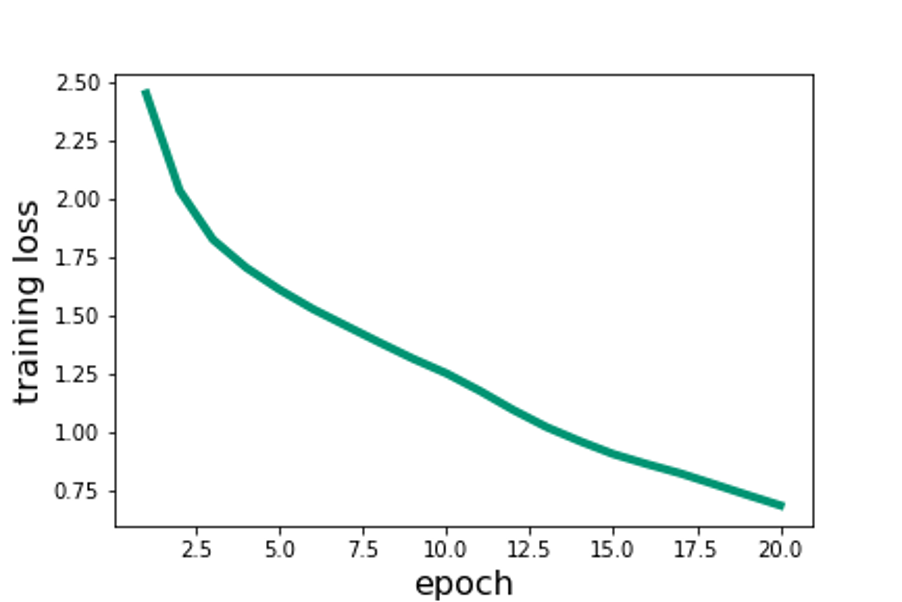
\includegraphics[width=7in]{FVLR.png}
\end{center}
\caption{\label{fig:FVLR}
Learning curve for Flicker30K data with the VGG16 model extracted features.}
\end{figure}

\begin{figure}[h!]
\begin{center}
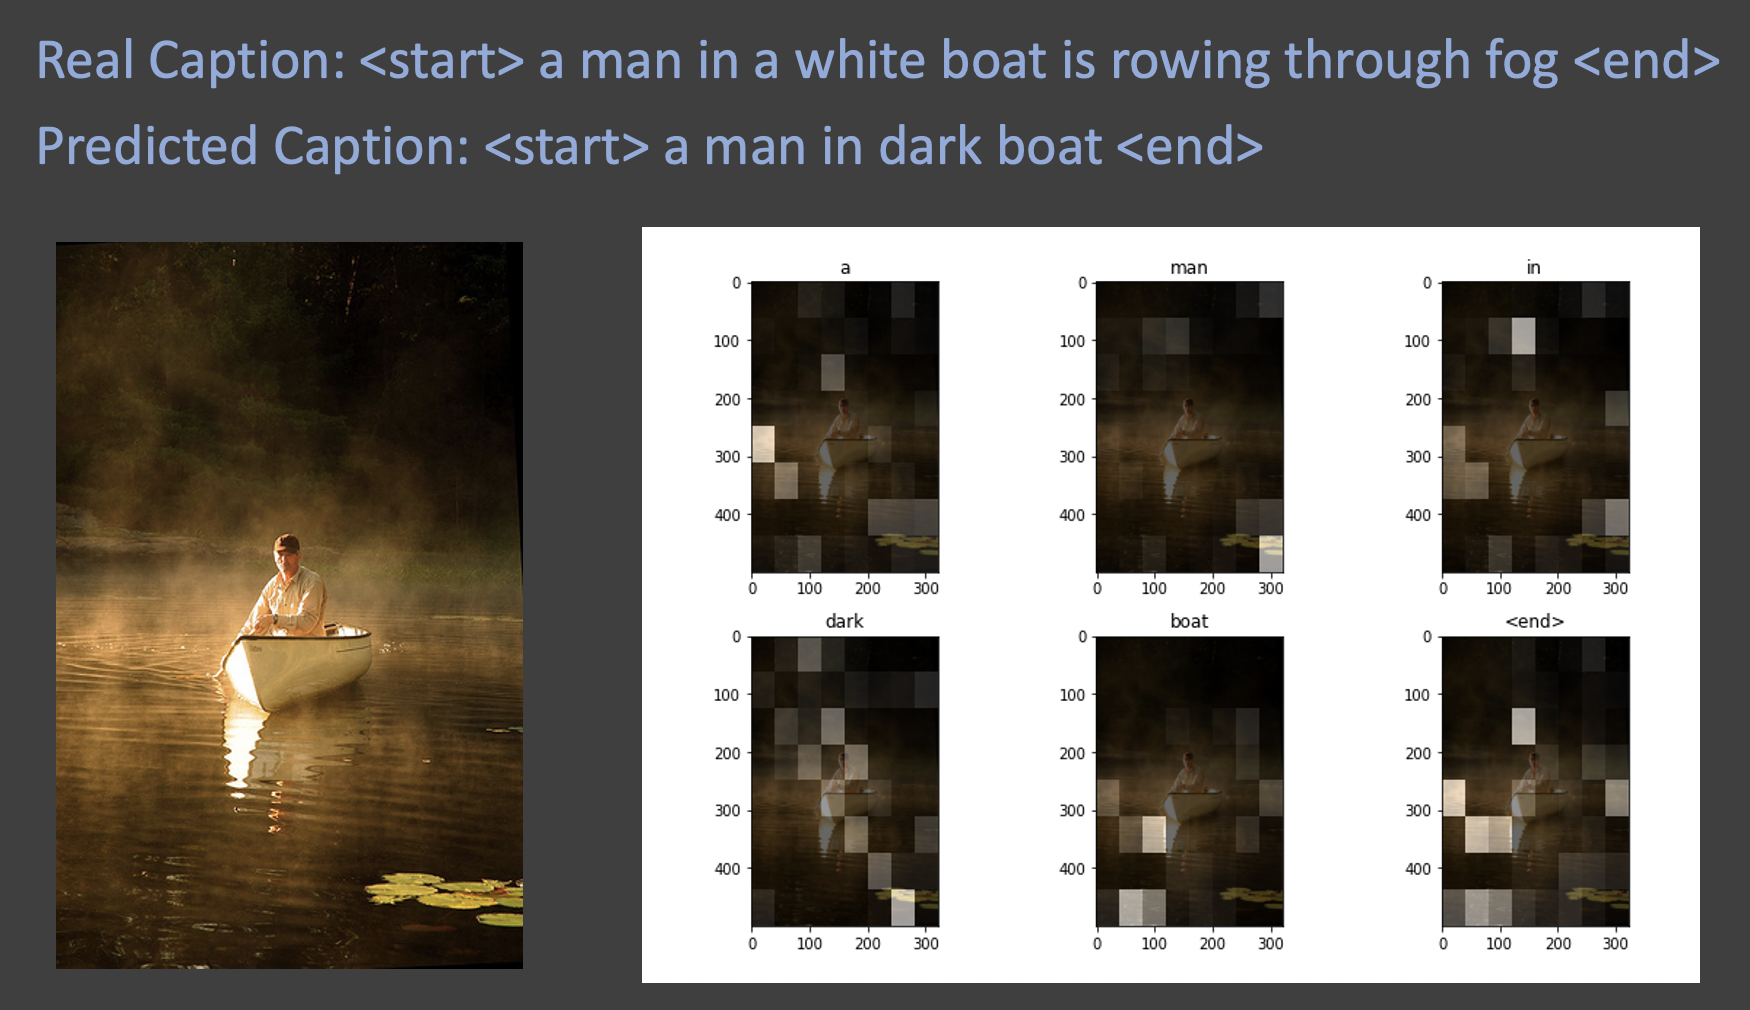
\includegraphics[width=7in]{FV_1.png}
\end{center}
\caption{\label{fig:FV_1}
A sample image with real and predicted caption (with vgg16 image model) along with the attention plot visualizing the part of the image responsible for the prediction.}
\end{figure}

%%%%%%%%%%%%%%%%%%%%%%%%%
\subsection{Flicker30K dataset with Inception V3 pretrained model}
\label{sec:imfeat}
%%%%%%%%%%%%%%%%%%%%%%%%%

Next, we train the Flicker30K dataset with the inception v3 pretrained model generated image features. We also trained the model for 20 epochs and the run time of this model is roughly similar to the runtime of the previous model. In Figure \ref{fig:FILR}, the learning curve shows that we can still train the model to improve the performance even further. In Figure \ref{fig:FI_1} \& \ref{fig:FI_2}, we show this model predicted caption and the corresponding real caption and the images. For the 1st image, the model is capable of extracting some major components from the image to describe it reasonably well but it fails to describe the fine detail present in the image. In the 2nd image, the model produced a different version of the caption; however, considering the fact that it was able to detect that a boy is waterskiing with his hand shows the model's impressive capacity to be able to understand the context of the image.

\begin{figure}[h!]
\begin{center}
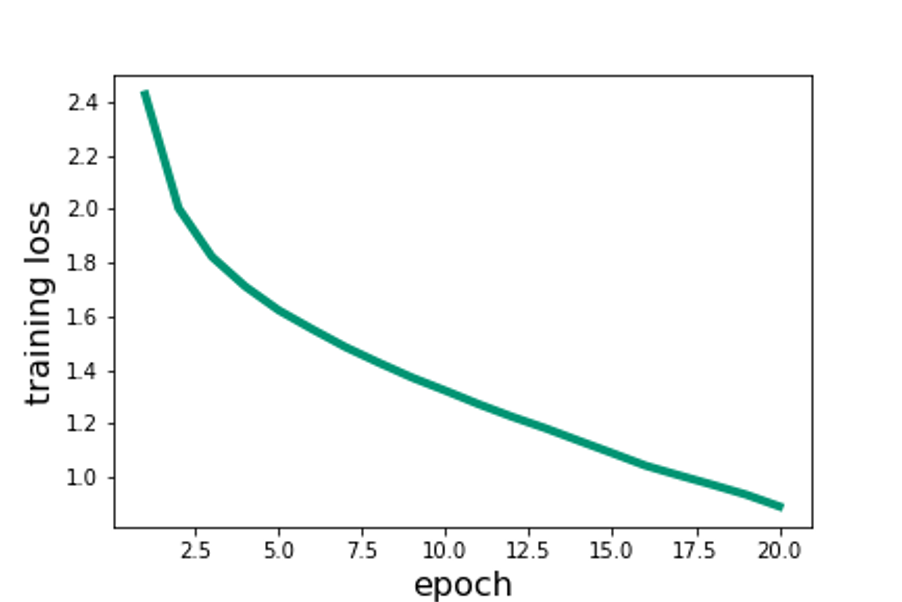
\includegraphics[width=7in]{FILR.png}
\end{center}
\caption{\label{fig:FILR}
Learning curve for Flicker30K data with the inception v3 model extracted features.}
\end{figure}

\begin{figure}[h!]
\begin{center}
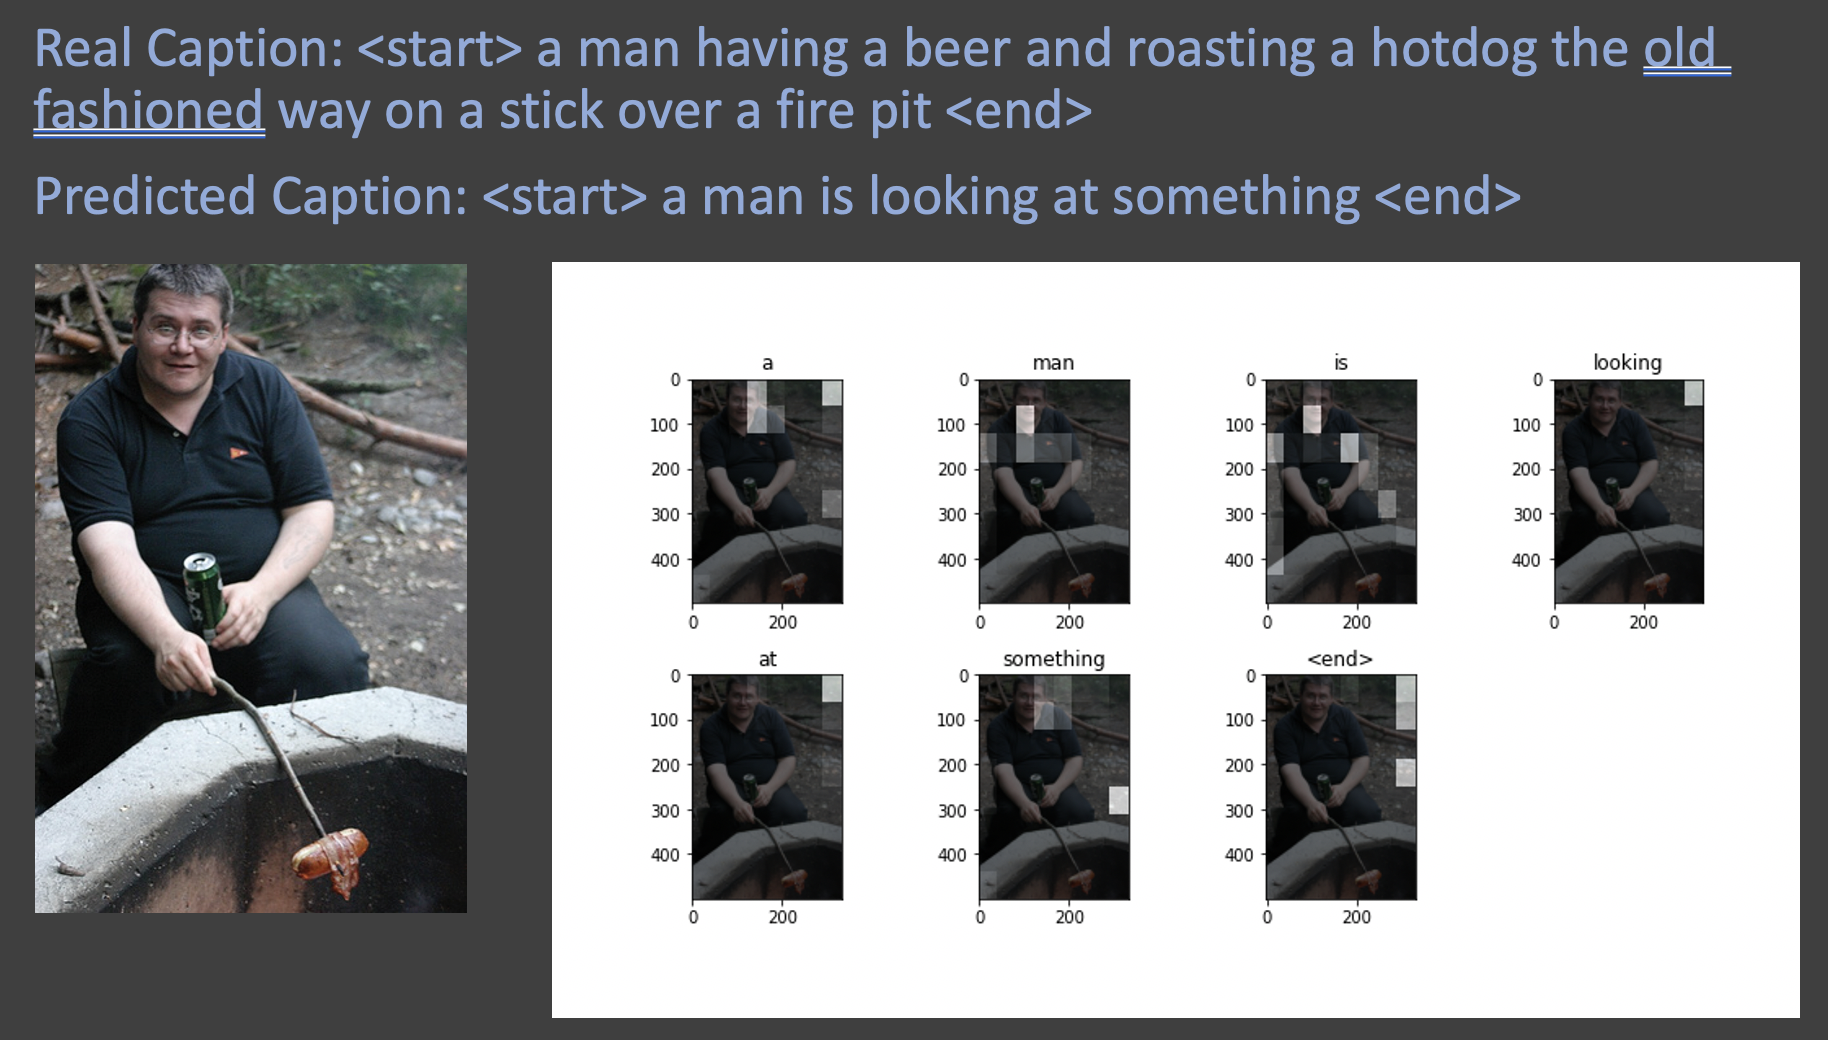
\includegraphics[width=7in]{FI_1.png}
\end{center}
\caption{\label{fig:FI_1}
A sample image with real and predicted caption (with inception v3 image model) along with the attention plot visualizing the part of the image responsible for the prediction.}
\end{figure}

\begin{figure}[h!]
\begin{center}
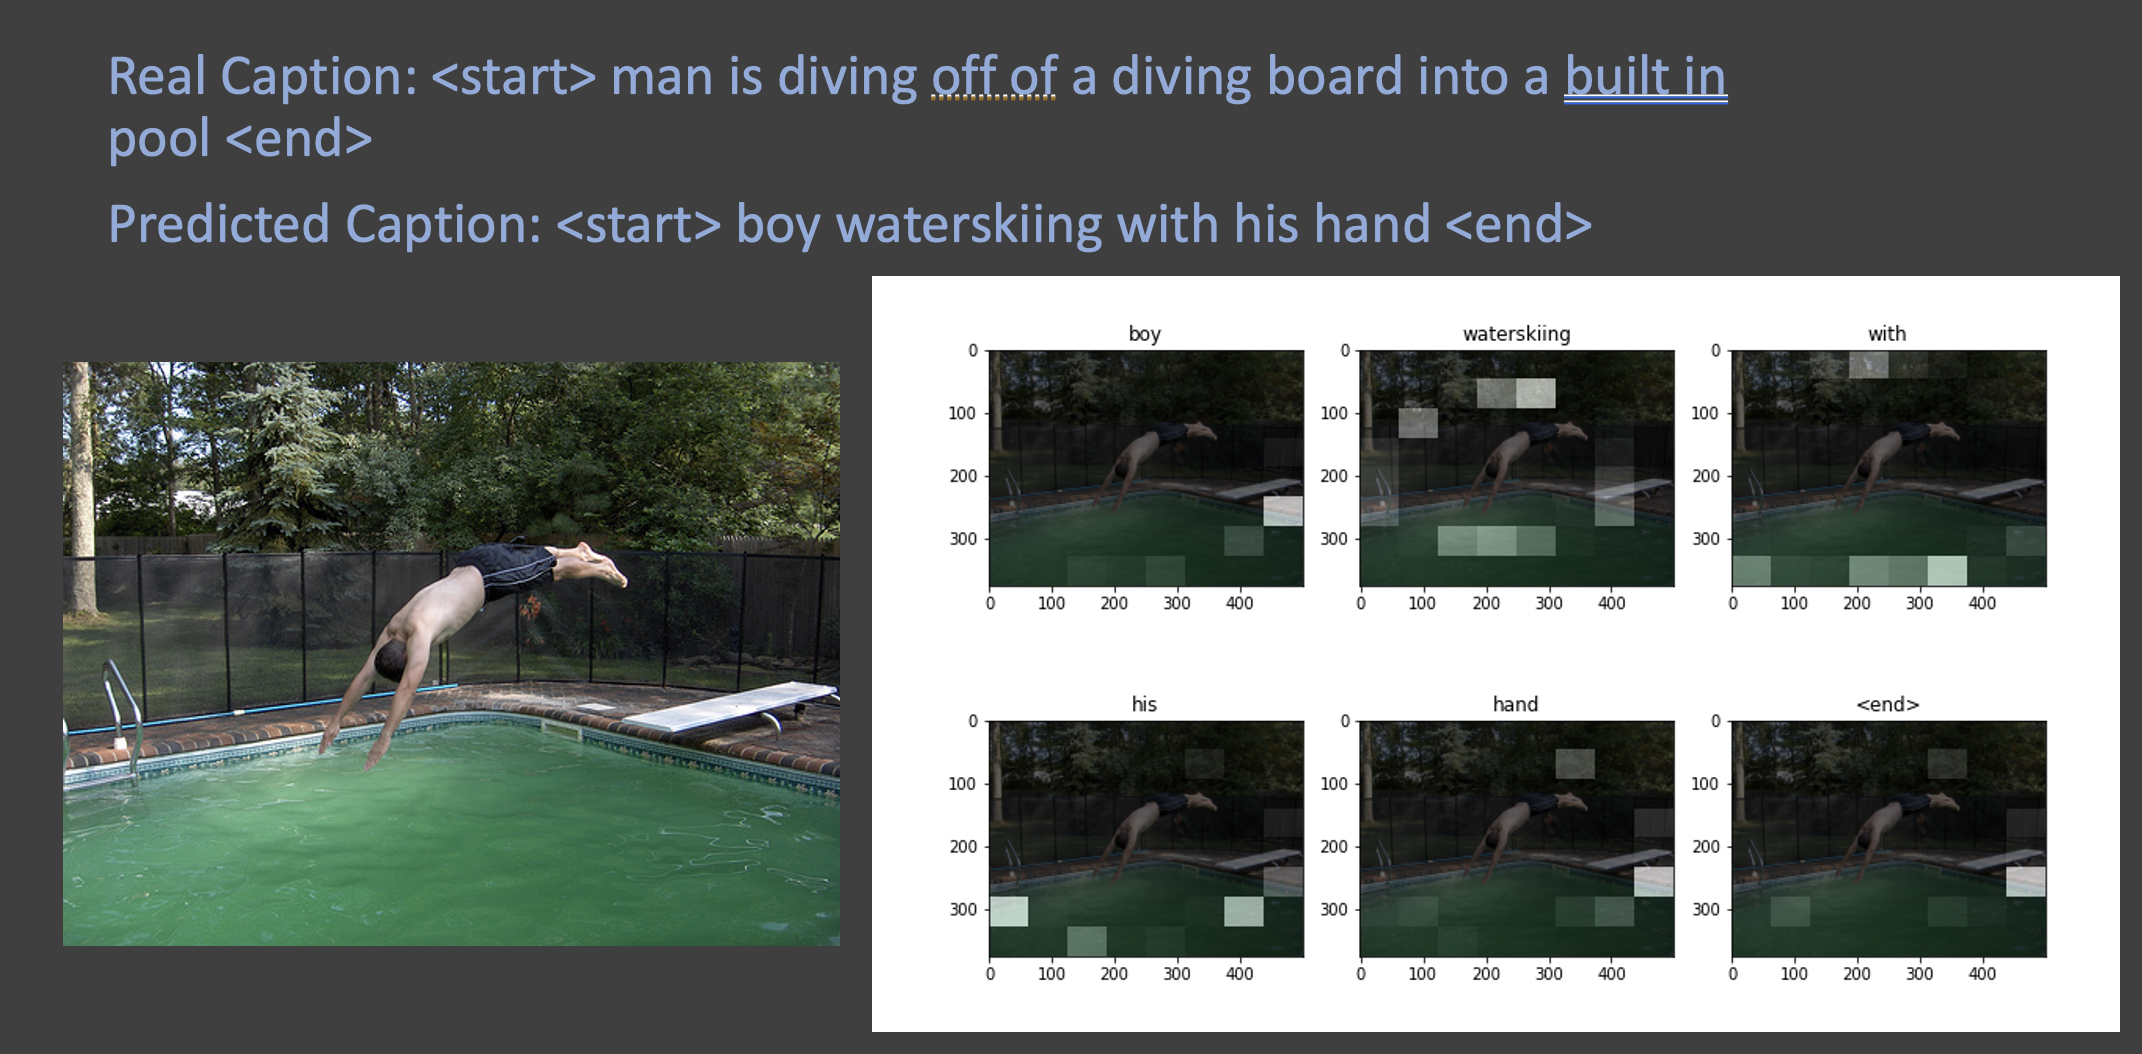
\includegraphics[width=7in]{FI_2.png}
\end{center}
\caption{\label{fig:FI_2}
A sample image with real and predicted caption (with inception v3 image model) along with the attention plot visualizing the part of the image responsible for the prediction.}
\end{figure}

%%%%%%%%%%%%%%%%%%%%%%%%%
\subsection{MS-COCO dataset with VGG16 pretrained model}
\label{sec:imfeat}
%%%%%%%%%%%%%%%%%%%%%%%%%

Having successfully trained model for the Flicker30k dataset, we turned our attention to training the MS-COCO dataset with the VGG16 pretrained model. We trained the model for 20 epochs as usual, but here in Figure \ref{fig:CVLR} it is obvious that the learning curve almost reached the plateau. Most likely due to the larger data size (about $30,000$ iamges were trained), the training was better than the Flicker30K dataset. In Figure \ref{fig:CV_1}, we show a sample MS-COCO image with the real and predicted caption. Similar to what we saw earlier with the Flicker30K dataset, the model focused on finding the simplest truth to describe the image rather than trying to find the fine detail.

\begin{figure}[h!]
\begin{center}
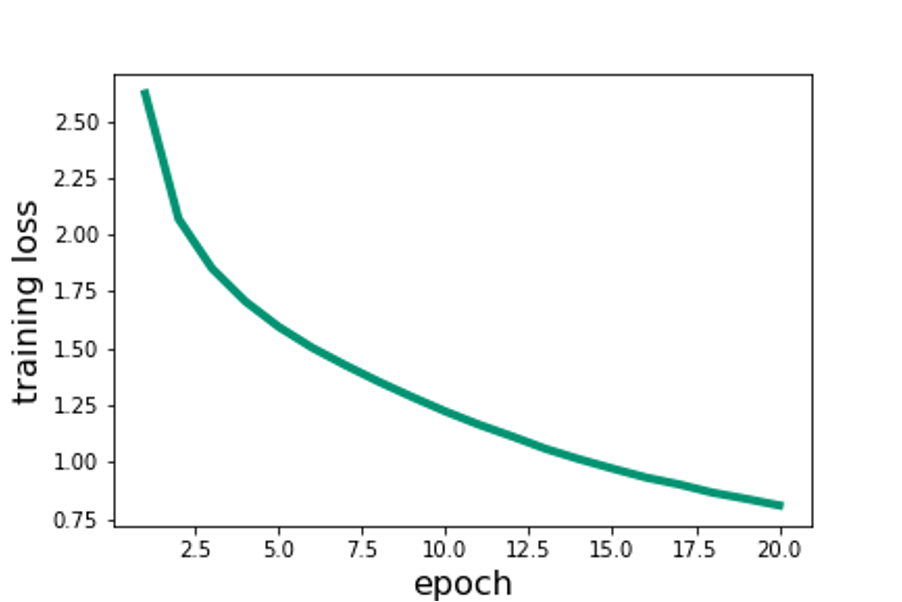
\includegraphics[width=7in]{CVLR.png}
\end{center}
\caption{\label{fig:CVLR}
Learning curve for MS-COCO data with the vgg16 model extracted features.}
\end{figure}

\begin{figure}[h!]
\begin{center}
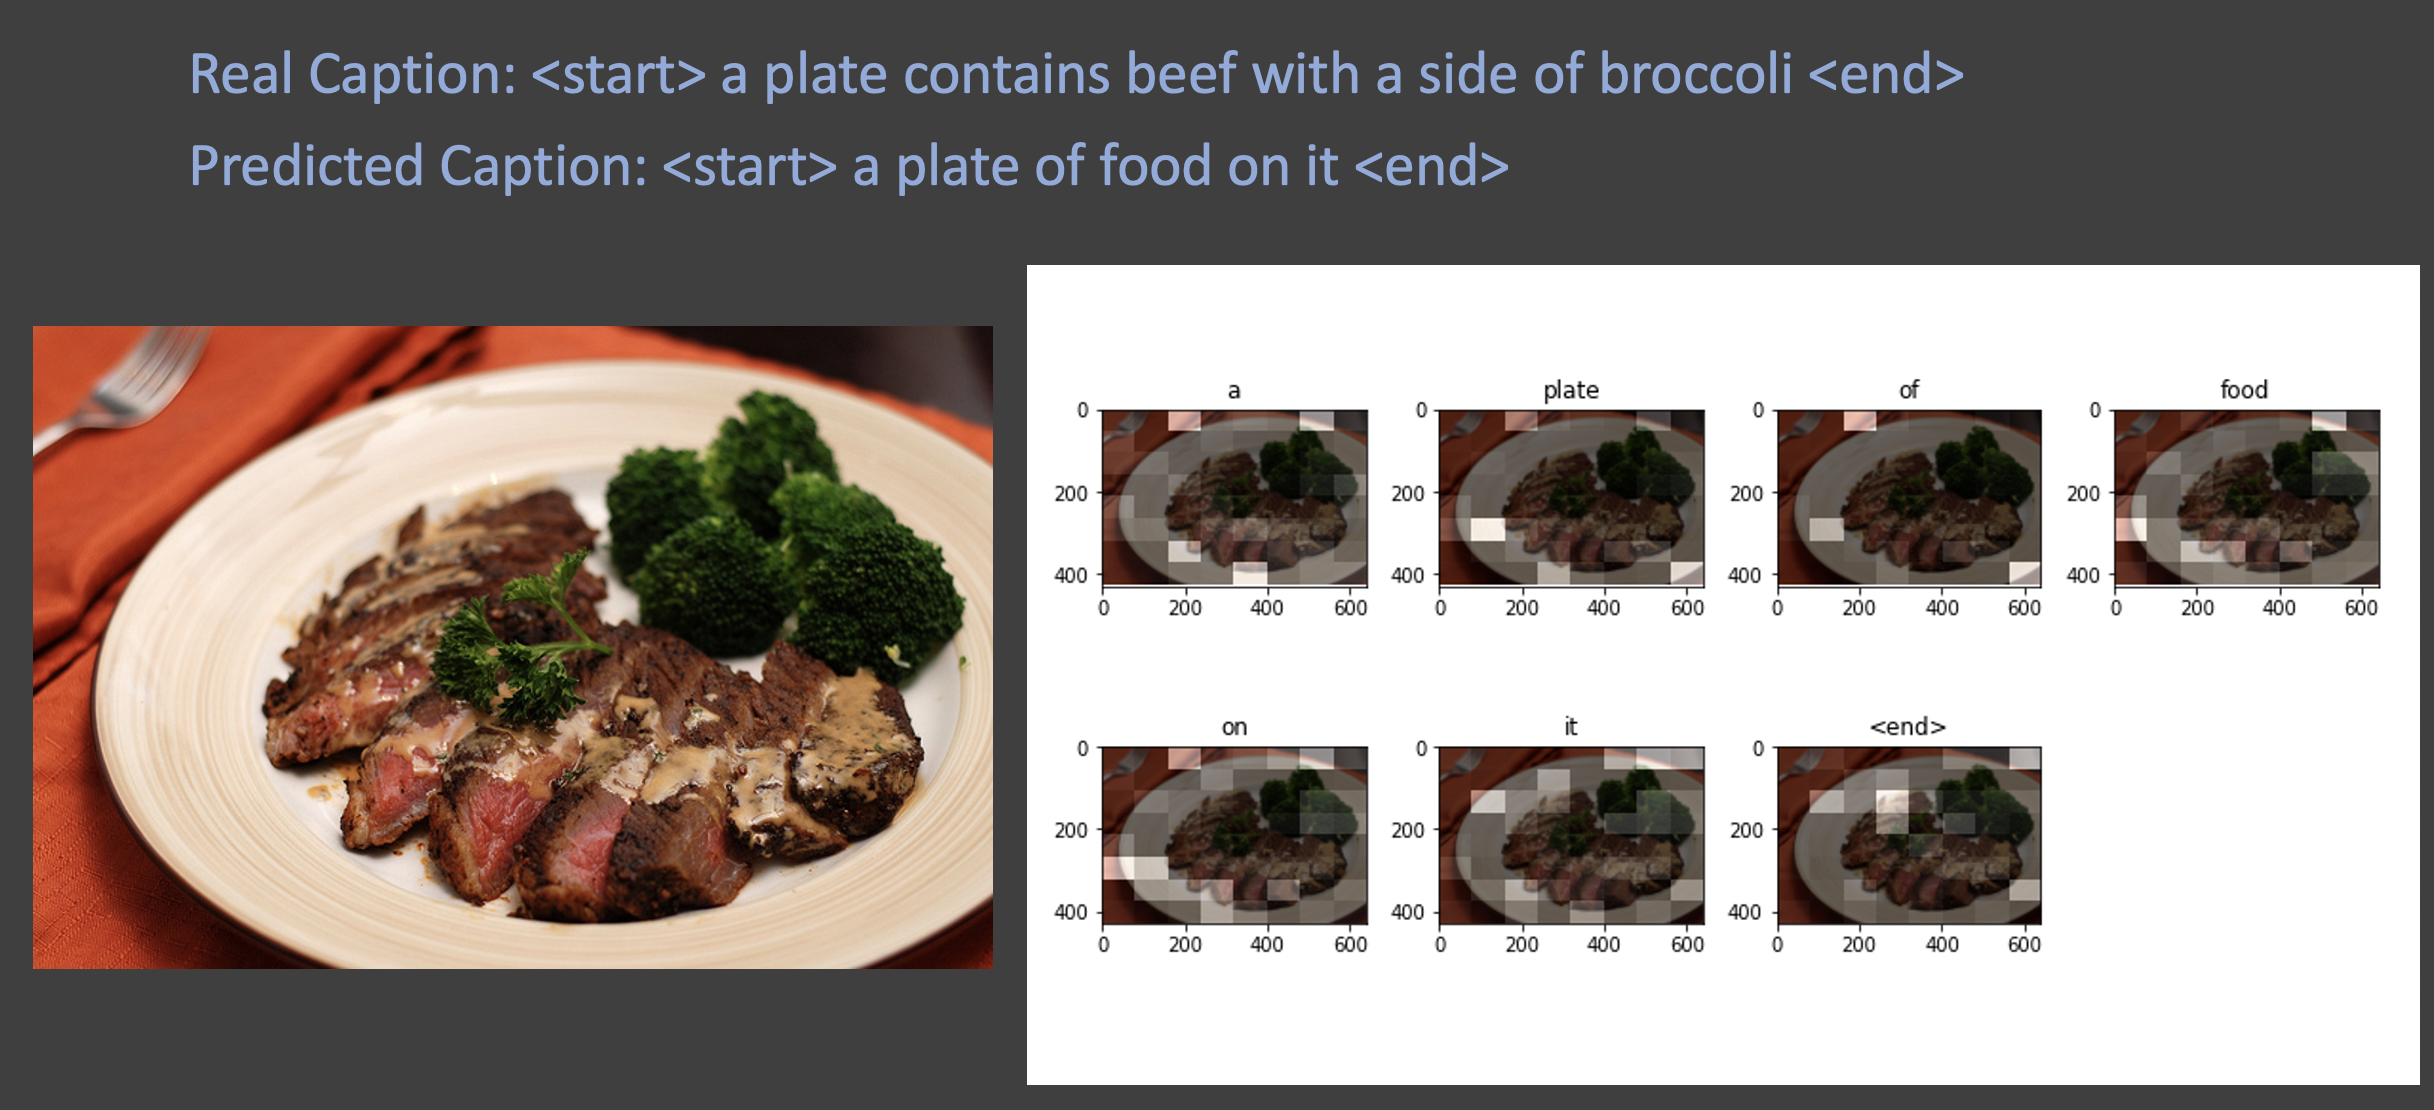
\includegraphics[width=7in]{CV_1.png}
\end{center}
\caption{\label{fig:CV_1}
A sample image with real and predicted caption (with vgg16 image model) along with the attention plot visualizing the part of the image responsible for the prediction.}
\end{figure}

%%%%%%%%%%%%%%%%%%%%%%%%%
\subsection{MS-COCO dataset with Inception V3 pretrained model}
\label{sec:imfeat}
%%%%%%%%%%%%%%%%%%%%%%%%%

Next, we trained the model with the inception v3 model generated image features. The training loss after 20 epochs seems reasonable. The learning curve (Figure \ref{fig:CILR}) is almost reached the convergence. The BLEU score on the holdout test set is about $0.73$, which can be considered very good as the highest possible BLEU score is $1.00$. In both Figure \ref{fig:CI_1} \& \ref{fig:CI_2}, it is obvious that the model is very well adapted to find animal in the images without any problem. In almost all the cased, the model suffered from simplification of the generated iamge caption. Most likely, we need to change the architecture or the loss function, to force the model to learn complex feature description. Notebooks for the machine learning model training can be found \href{https://github.com/mamunm/iamge_caption_generator/tree/main/notebooks}{in this folder}.

\begin{figure}[h!]
\begin{center}
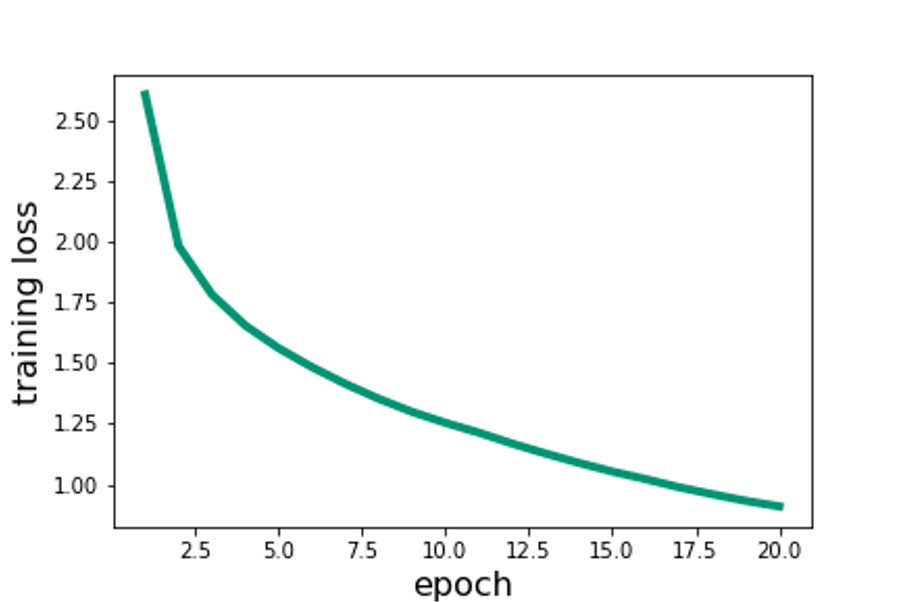
\includegraphics[width=7in]{CILR.png}
\end{center}
\caption{\label{fig:CILR}
Learning curve for MS-COCO data with the inception v3 model extracted features.}
\end{figure}

\begin{figure}[h!]
\begin{center}
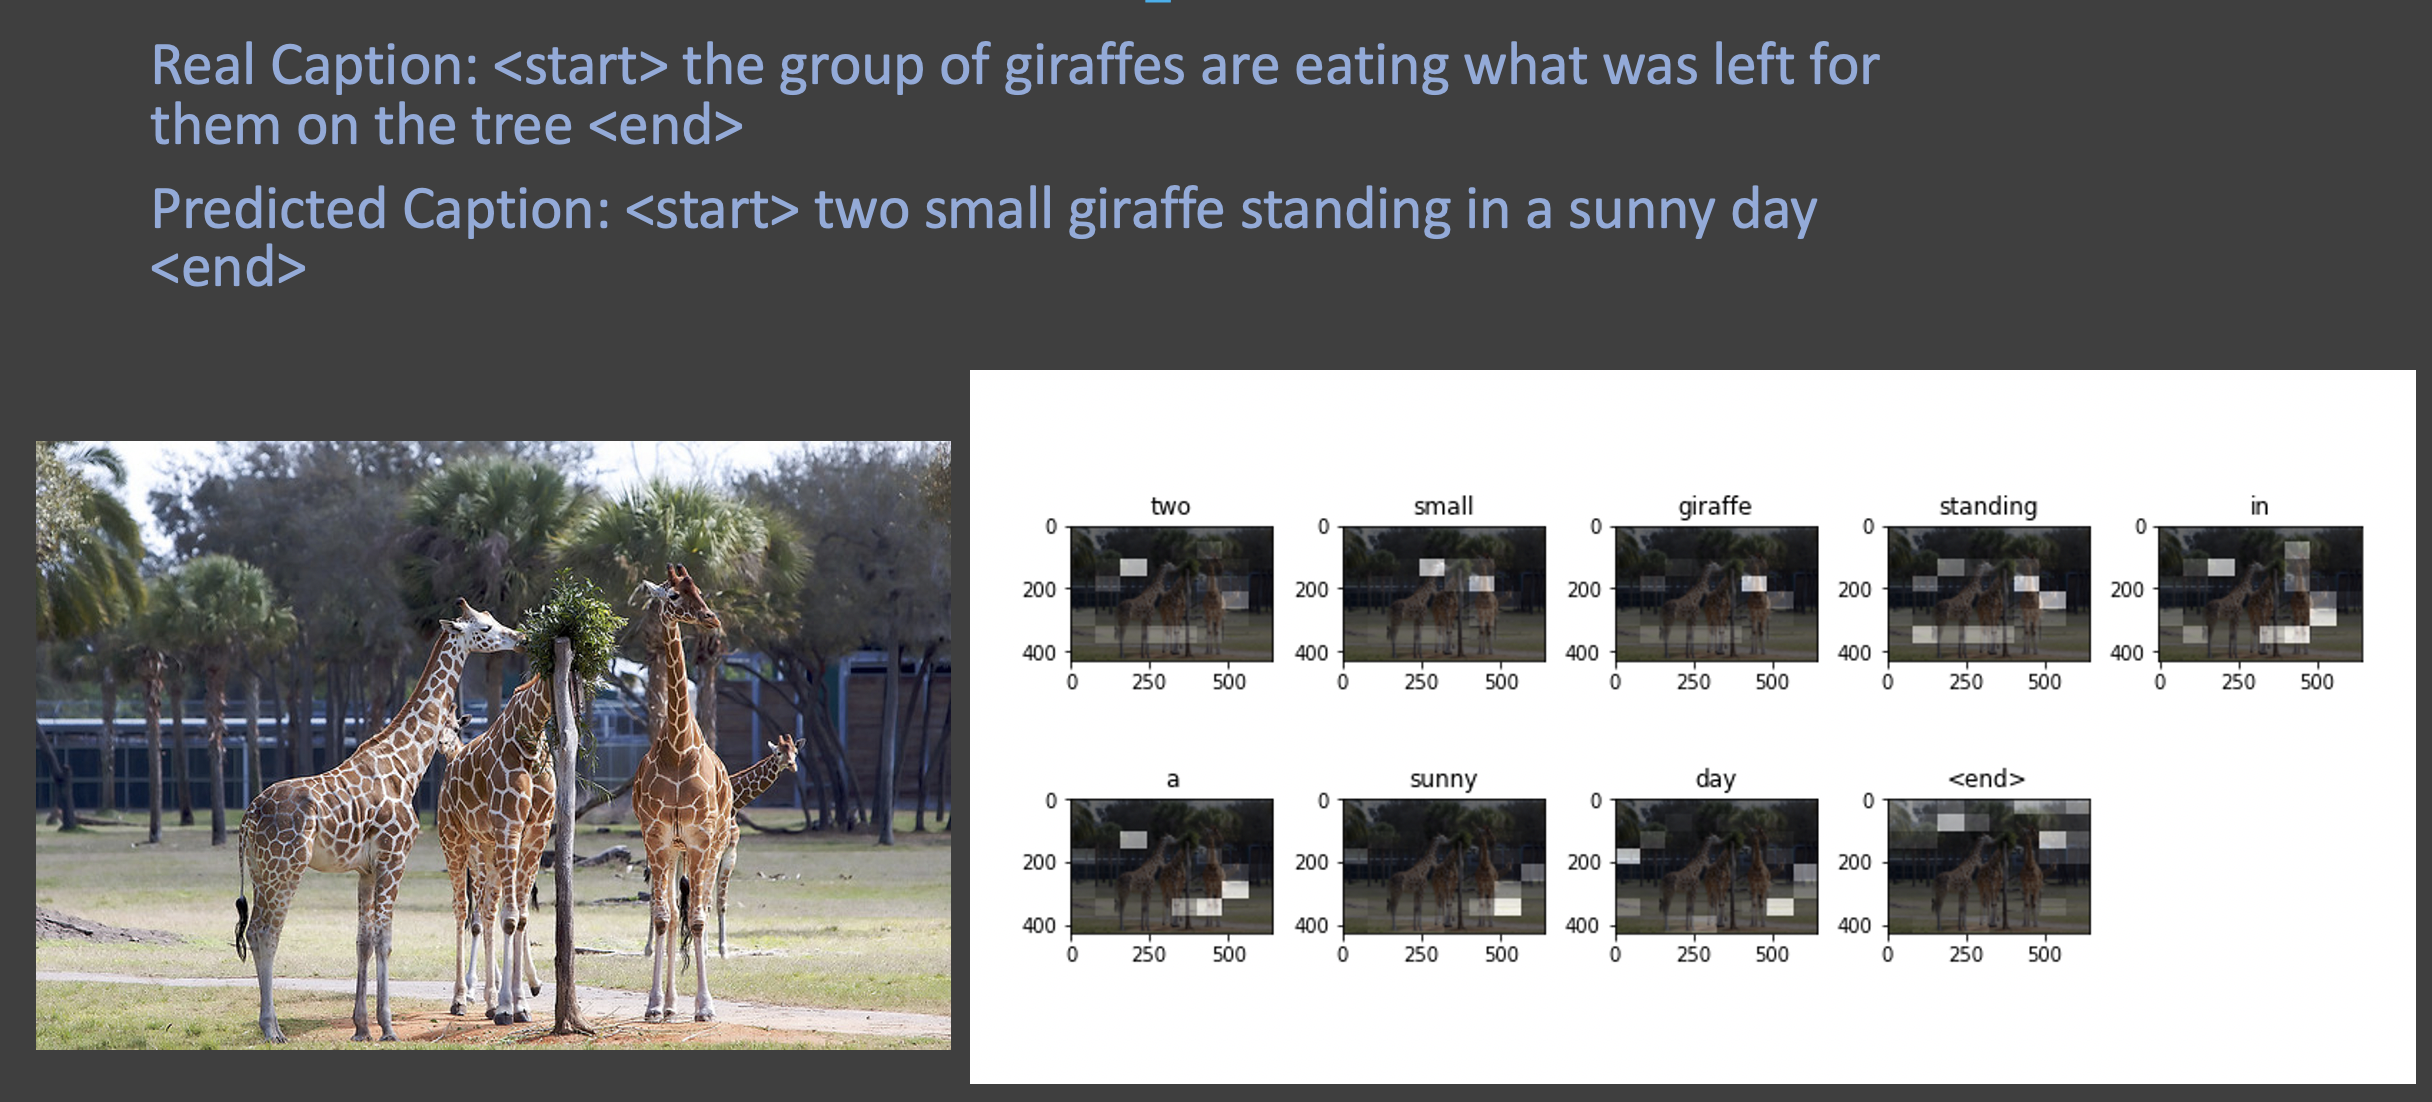
\includegraphics[width=7in]{CI_1.png}
\end{center}
\caption{\label{fig:CI_1}
A sample image with real and predicted caption (with inception v3 image model) along with the attention plot visualizing the part of the image responsible for the prediction.}
\end{figure}

\begin{figure}[h!]
\begin{center}
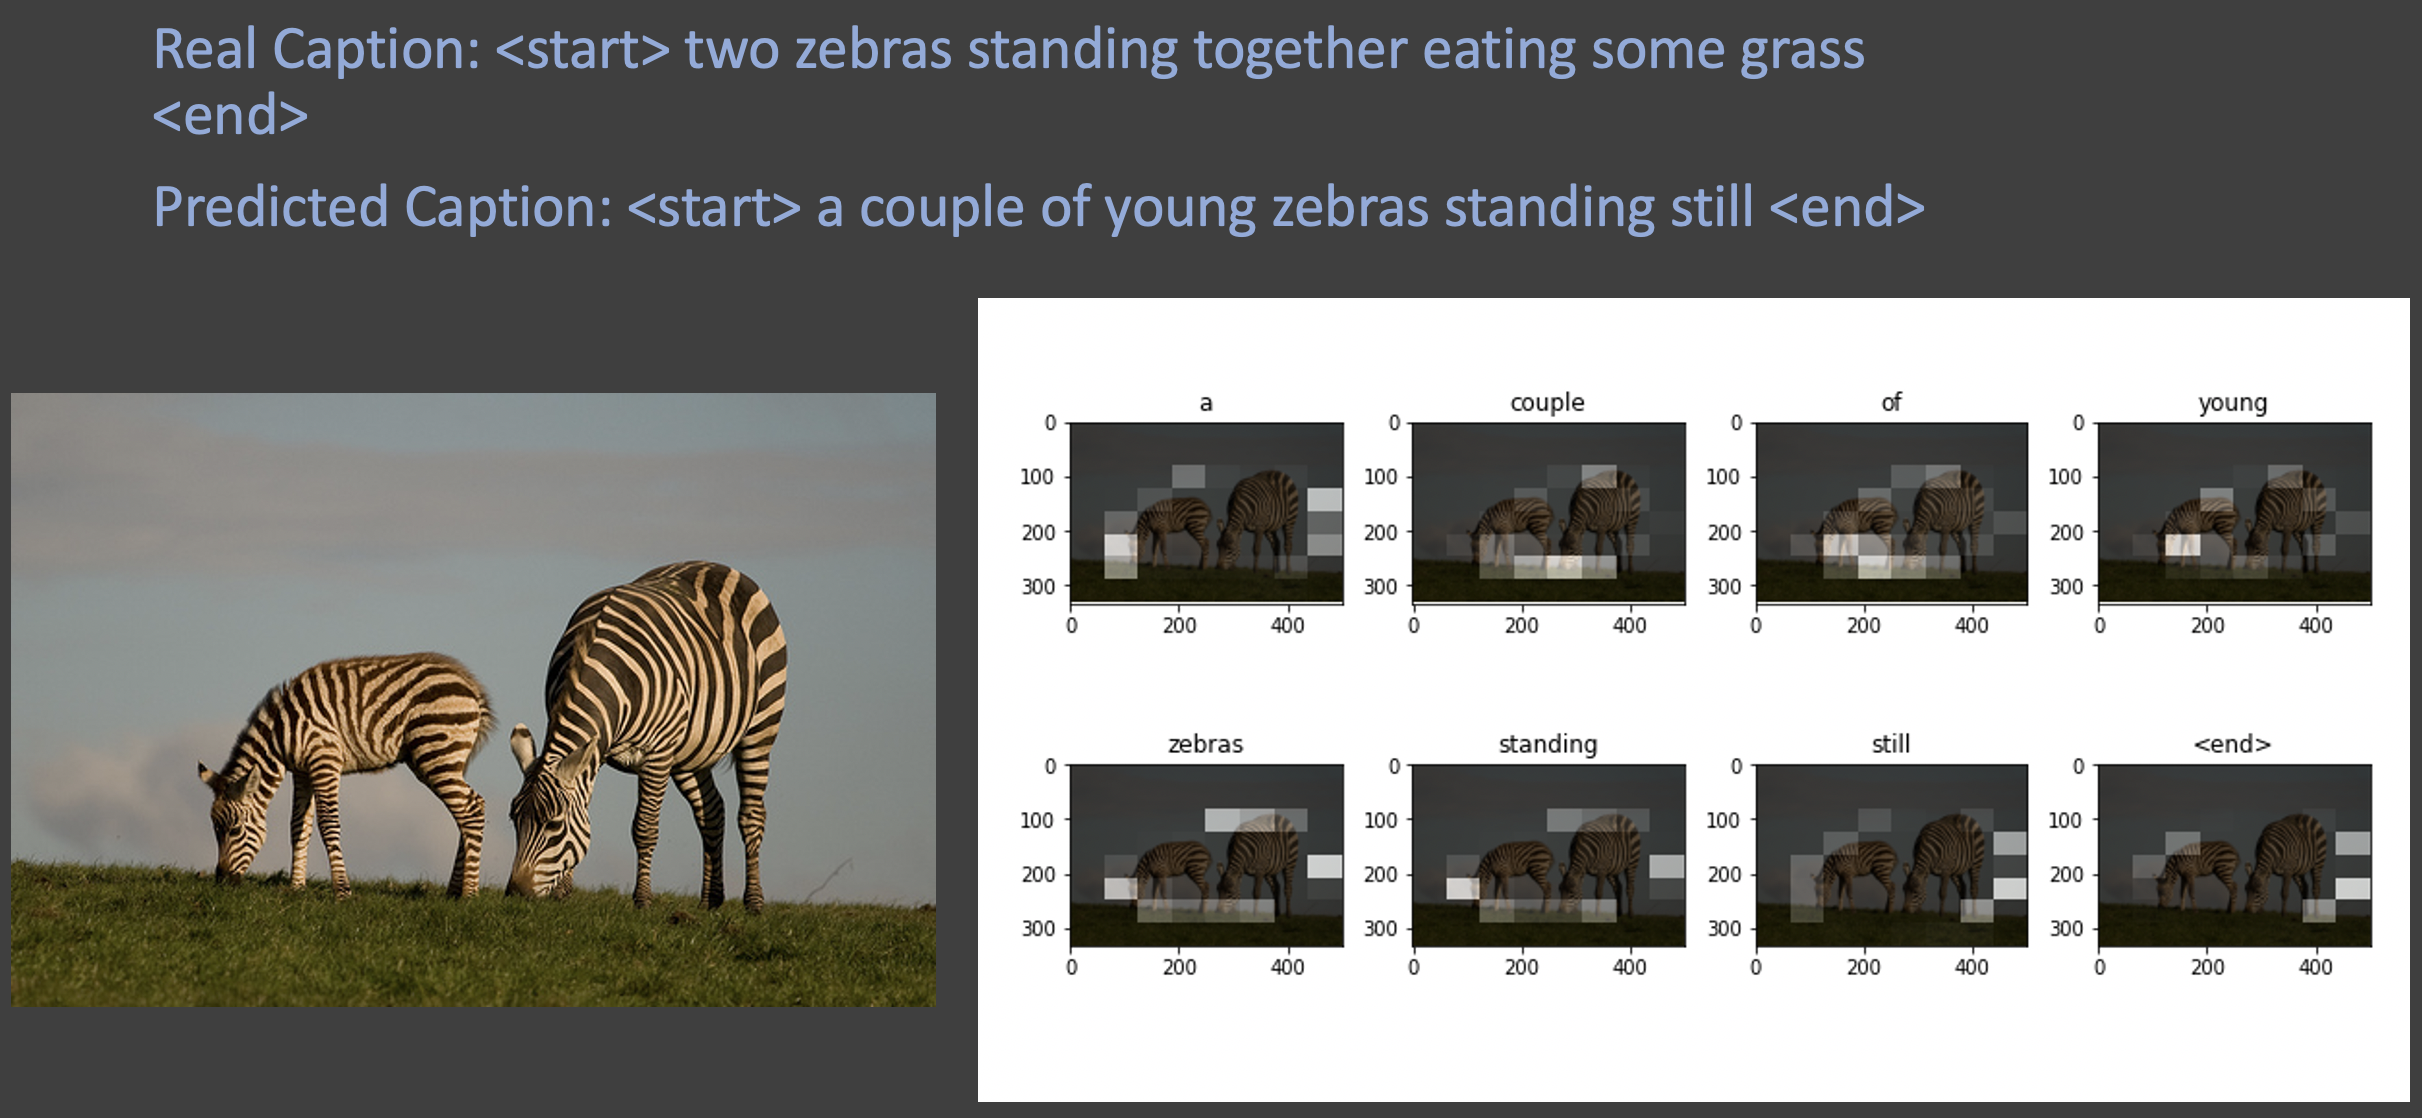
\includegraphics[width=7in]{CI_2.png}
\end{center}
\caption{\label{fig:CI_2}
A sample image with real and predicted caption (with inception v3 image model) along with the attention plot visualizing the part of the image responsible for the prediction.}
\end{figure}

\section{Conclusion}
%%%%%%%%%%%%%%%%%%%%%%%%%%%%%%%%%
In this work, we demonstrate an image caption generator model from the publicly available dataset. Even though the model is pretty rudimentary, but it is still can perform reasonably well to generate caption for images drawn from the same data distribution. Below are some ideas for future work:

\begin{enumerate}
\item Using different pre-trained image model.
\item Using pre-trained language model for word embedding.
\item Use a larger dataset.
\item Build a web-app for customer to interact with the final model.
\end{enumerate}

\end{document}
%%%%%%%%%%%%%%%%%%%%%%%%%%%%%%%%%%%%%%%%%%
